\documentclass{article}
% General document formatting
\usepackage[margin=0.7in]{geometry}
\usepackage[parfill]{parskip}
\usepackage[utf8]{inputenc}
\usepackage{subfig}         % side-by-side figures 
% Related to math
\usepackage{amsmath,amssymb,amsfonts,amsthm}
\usepackage{graphicx}
\usepackage{natbib}
\bibliographystyle{unsrtnat}


% \usepackage[math]{kurier}
\usepackage{setspace}       % \onehalfspacing and \singlespacing
\newcommand\be{\begin{equation}} % shortcut to start eq envs 
\newcommand\ee{\end{equation}}   % shortcut to end eq envs
\newcommand\ol{\overline}        % shortcut to draw overline 
\newcommand\bra{\langle}
\newcommand\ket{\rangle}

\begin{document}

\title{don't know}
\author{Kevin Pierce}
\maketitle
\section{abstract}
words

\section{What is the problem?}

Under typical conditions, sediment grains move intermittently in a sequence of start-stop motions, rolling, bouncing, and sliding along the bed under the action of the water flow.
When tracer grains are stationary, they may be buried by other sediment which comes to rest on top of them, leading to long periods of residence over which these buried tracers do not move.
Eventually, the sediment above these buried tracers can be transported away, exposing the previously buried tracers to the water flow again. 
The time period between the burial of a stationary tracer and its emergence on the bed surface again, we call the residence time. 
The residence time is not a deterministic quantity, but because it links to the process of sediment transport, its statistics should relate to the characteristics of sediment transport. 
Our directive is to calculate the burial time distribution in terms of the erosion and depostiion rates of sediment transport. 

\section{What do we know about it?}

We know the burial time is a stochastic variable. 
We know it is the reason for anomalous diffusion. 
Bed elevations lie on a normal distribution
burial times are expected to be ... 
sediment transport is really a stochastic process


\section{What are the gaps and limitations of our knowledge?}

We do not know how the characteristics of sediment transport relate to the burial time or its distribution. 

\section{How can we solve this?}

\section{Make a physical diagram of the problem}

\section{What are your assumptions?}

\section{Solve the problem.}



\section{Paper Notes}

\begin{itemize}
\item Nakagawa and Tsujimoto 1980:
These authors develop a birth-death process where-in the bed elevation changes in discrete steps in order to describe the incipient development of bed elevation changes. The master equation is like $\partial_t p(m,t) = \lambda p(m+1,t) + \sigma p(m-1,t) - (\lambda + \sigma) p(m,t)$ from which they find $\sigma_m^2 \propto t$, a result which agrees with their experiments on a flat bed evolving into a dune bed with time, for short times only. Then the scaling of $\sigma_m^2$ saturates. In any case, it's a very similar type of model as the elevation component of yours. 

\item Yang and Sayre 1971 "Stochastic model for sand dispersion ":
Strongly related to Einstein 1937, but more general. In relation to the bed elevation issue, they relate the resting time pdf to bed elevation, but not in context of burial. 
They consider that, across a bed of dunes, regions of low elevation have a relatively larger resting time, while regions of high elevation have a relatively higher resting time. 
They marginalize the resting time pdf over bed elevation like $p_{T|z}(t,z)$ and they claim the empirical exponential resting time distribution $p_T(t)$ should result from a convolution integral $p_T(t) = \int dy p_{T|Y}(t,y)p_Y(y)$, where $p_Y(y)$ is the probability of deposition at elevation $y$. 
They highlight the entrainment rate is the inverse of the resting time, $p = 1/T_r$. 

\item Yano et al 1969 "Studies on the Sand Transport in Streams with Tracers": 
The authors formulate an Einstein-like (1937) formula from a stronger physical concept, and they supported their formulation with tracer experiments on colored sand. Essentially, they hold the same assumptions as Yang and Sayre, that travel distance is gamma distributed while resting time is gamma distributed. However, they clarify these distributions by introducing further quantites. 
This means the resting time, or the waiting time for a single step, is exponential; and similarly the travel length in a single step is exponential. These results stem from more general considerations. 
For example, they define $\lambda_1$ as the entrainment probability per unit length, and they write a master equation 
$$ \frac{dp(n;x)}{dx} = -\lambda_1 p(n;x) + \lambda_1 p(n-1;x)$$ for the change by $n$ steps, so they get a Poisson distribution for the distance traveled in $n$ steps: 
$$ p(n;x) = e^{-\lambda_1 x} (\lambda_1 x)^n/{n!}.$$
They state that $1-\sum_{i=0}^{n-1} p(n;x)$ is the probability that the particle remains at $x$ after $n$ steps, from which they determine the pdf of travel distance as 
$$ f(x;n) = \lambda_1 e^{-\lambda_1 x}(\lambda_1 x)^{n-1}/\Gamma(n). $$
This is a nice analysis supporting a gamma-distributed step length which emerges from a constant entrainment probability within a unit length of bed. 
I'm not 100 percent sure I understand it. 
They do a very similar analysis on entrainment probability per unit time to find a gamma distributed resting time distribution. 
They convolve these distributions together to find the same type of result as Einstein involving the modified Bessel functions and an exponential factor. 
They find tracer diffusion scales like $t$ -- normal diffusion. 
Using a thickness of bedload layer concept, $t_l$, and evaluating the time derivative of the mean position at time $t$, they compute a drift velocity, and write the bedload transport rate as $q_s \propto t_l U_D$, in the same manner as Yang and Sayre. 

\item Yano et al 1969 " Tracer studies on the movement of sand and gravel": 
This is a more brief conference proceedings of the other Yano paper. The other one is much better. Although this contains the significant information, it leaves too many gaps for someone only as smart as me to really fill. 

\item Sawai 1987 "Dispersion of bed load particles":
These things are, by 1987, pretty clearly fact: the active layer is about a grain diameter thick; coarser particles are more exposed; coarser particles move faster than fine particles, meaning they disperse more rapidly; the change in bedload rate with discharge is attributed to change in activity, not velocity.
These authors in their abstract make an attractive statement: "bed level variation exhibits two opposite effects. The increase of the degree of exposure accelerates dispersion, but the reduction of shear stress decelerates it."
They state the compound exponential-exponential model of Einstein 1937 or Sayre and Hubbell 1964 is totally adequate at least for early times of dispersion on uniform sand. 
They state dunes imply the step length deviates from exponential while the resting period stays exponential. 
They state the rest period for a particle deposited on the dune face or in the eddy region downstream of it remains buried until it is exposed again by the advance of the dune, in which case the rest period is the duration during which a particle is buried. 

Nakagawa and Tsujimoto 1979 in Japanese apparently holds the rest period on an equilibrium flat bed is a gamma distribution, rather than expoenntial. They argue this is because of bed elevation fluctuations: the mean rest period over elevations is different for each elevation. This is essentially what Yang and Sayre 1971 said... except they held the overall rest period distribution remained exponential, while they did not pin down the form of the elevation conditional rest period distribution. 

Sawai does not really consider burial. He instead only considers colored tracers on the surface relative to a mean elevation. 
He finds a somewhat normal distribution of 'exposure' or elevation of tracer particles. 
He plots entrainment probability versus exposure and notes a marked drop in entrainment probability with relative exposure. This is an important conclusion which supports your model. Specifically, it supports the formula you wrote: $\lambda(m) = \lambda_0(1+z_1z(m)/(2l)^2). $ It does not really support the opposite equation: $\sigma(m) = \sigma_0(1-z_1z(m)/(2l)^2)$, although it does not refute it either. 

I suspect tracer burial and loss was more common for tracers which deposited at lower exposures, meaning few datapoints from lower exposures were collected, implying the skew in the exposure distributions. 
They do a computer model which uses their empirical relationships for the exposure dependence of pickup probability. 
An important conclusion: "The expected value of the pickup rate seems to correspond to a considerably exposed condition, with a degree of exposure of about 0.5."
The degree of exposure is the bed elevation minus the mean bed elevation over the particle diameter. 
So they claim the expected entrainment probability per unit time corresponds to the value at positive exposure.. I guess this makes sense, right? 
\textbf{"for uniform material, the pick up rate is approximately linearly related to the degree of exposure"} KEY QUOTE 
For nonuniform material, the pick up rate varies exponentially with the degree of exposure and differs by a factor of 100 between the top and bottom of the active layer. 


\item Sayre and Conover 1967 "General two-dimensional stochastic model for the transport and dispersion of bed-material sediment particles": 
This paper indicates that Sayre et al definitely consider the distribution $f_{T|Y}(t,y)$ exactly as you do. It's the probability of a rest of length $t$ given the resting started at elevation y. They interpret it as burial and re-exposure, and they show a nice figure of it (fig 2.) Their model is impractical to apply. 
They do not attempt to constrain the burial time distribution. They do not attempt to relate it to dune migration or the timescales of sediment transport. They definitely do consider the entrainment probability to be 1/T, where T is the resting time, including burial. This is all a bit confusing, like trying to decipher ancient texts. 

\item Vukmirovic and Junior, 1976 "bed load movement as a random process": 
Very nice paragraph descriping phenomenology of sediment motion. 
May need to read Grigg 1970. 
This paper considers (1) the number of deposition events in a time interval; (2) the number of deposition events over a travel distance; (3) the time required for n double cycles (using the Einstein terminology); the distance traveled during n double cycles. 
Pretty nightmare paper. Messy. Apparently more general than Yang and Sayre-- inhomogeneous in time.
All in all, not very good. Pretty terse and not carefully phrased. More a statistics exercise than anything. 

\item Crickmore and Lean 1962 "The measurement of sand transport by means of radioactive tracers":
"particles in low levels in the ripples are at rest for a very much longer time than those in the upper levels so that the spread of the sand particles is much larger than is the case for fluid flow of the same mean velocity and depth." 
They discriminate section and plan. You should learn this difference; it is a geology terminology. 
"Statistical methods which ahve been developed for the analysis of moving random surfaces such as the surface of the sea can also be applied to the ripple surface, although it has been found that the bed elevations are not distributed normally about the mean." 
"It seems certain there exists a certain low level of movement below which troughs never penetrade provided the bed is subject to no net scour." 
 Are they suggesting the elevation distribution is skewed? 
They obtain bed elevation distribution by dewatering somehow. 
They get a very nearly Gaussian bed elevation distribution with perhaps a slight positive skew. They are definitely slightly assymmetric, but by a small degree. 
They are also measuring over space, and not through time. 

They develop a Poisson model considering that each particle has an equal probability $c$ of moving through $L$ in time $T$. Thus after time $T$, the spatial distribution of the cloud is $((1-c)*0 + c*L)*w$ or something. 
Anyway, they've made an Einstein-like model, too, which is quite surprising. 
\textbf{"In any particular core the activity decreased sharply above a certain depth, the tracer particles being undisurbed below this depth and nearly absent above it"} -- this sentence is in relation to taking core samples to determine that a max scour depth (or an $l$ value) is a well-defined quantity. 
good paper

\item Crickmore and Lean "The measurement of sand transport by the time-integration method with radioactive tracers": 
This is the followup to the previous paper by Crickmore and Lean. 
That was a space integration method. This is a time integration method. 
In this case, they do not move the scintillator. Previously, they moved it around. 
This is mostly a methods paper with some simple and outdated models of sediment dispersion. They develop a binomial model. Really, the previous paper is much better, although I get this was important when it was written. 
They do not really examine bed elevation. They do examine the depth of tracer mixing, but I don't get much from it. 
They do not discuss burial or timescales of burial. 


\item Wong and Parker 2007: 
They state \textbf{"the fraction of tracers moved per layer increases with excess shear stress as does the effective depth of tracers subject to entrainment"}, meaning that $l$ should scale with $\tau_*$.
They find bed elevations are very nearly normally distributed. 
"The total particle entrainment rate $E$ is obtained by ertical integration of the measured layer-specific entrainment rates. The entrainment rate of a given layer, however, must be normalized by the fraction of time the bed surface is actually at that layer." 
The fraction of time the bed surface is actually at layer $z$, $t_z/T$, is actually the probability that the bed is at height $z$. 
So they're saying the entrainment rate $E = \int dz p(z) E(z).$

They state entrainment and deposition rates at a point vary exponentially and they use their experimental data to support the entrainment rate scaling. 
Like me, they make the assumption that entrainment and deposition rate scalings are equivalent, because they have no data to contrary. 

They have excellent physical interpretations of the transport rate $q = El$. First, changes in transport with shear stress can be almost entirely associated with changes in $E$. I think Nakagawa and Tsujimoto say the same thing. At the same time though, as shear stress increases, so does the variance of bed elevation, meaning there is a higher probability for low relief areas on the bed, and a higher deposition rate. 
Accordingly, $l$ is decreased by shear stress, while $E$ is increased by shear stress. 
There is actually a bit of a competing mechanism here, but the net result is that shear stress may decrease travel distance in a way. 
Of course, it also provides more propulsion meaning there are less interactions with depressions on the bed surface, so probably shear stress still increases travel distance. 

They say an interesting thing about entrainment rates: "The entrainment rate should be independent of experiment duration"...
Since bed elevations change over experiment durations, what this really means is entrainment rates should be marginalized so that they become independent of bed elevations. Really, we should always write $E(z)$ instead of $E$. Certain times, ignoring bed elevation changes is a fine approach. This just means $E$ does not change appreciably with elevation $\Delta z = E \Delta t k a^3 \approx 0$. 

all in all, great paper. Highly important. 
There is a possibility that an exponential form for entrainment and deposition rates will not express a normally distrubted bedload rate....
I wonder? 


\end{itemize}




%\pagebreak
%\begin{figure}[h!]%
%    \centering
%    \subfloat[particle activity distribution]{{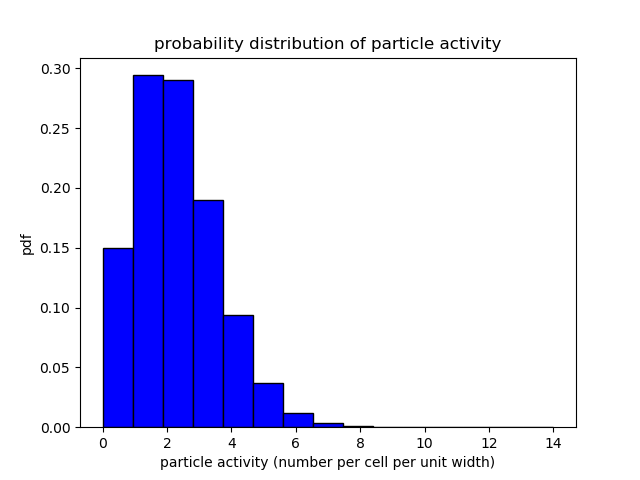
\includegraphics[width=0.45\textwidth]{activitypdf.png} }}%
%    \qquad
%    \subfloat[bed elevation distribution]{{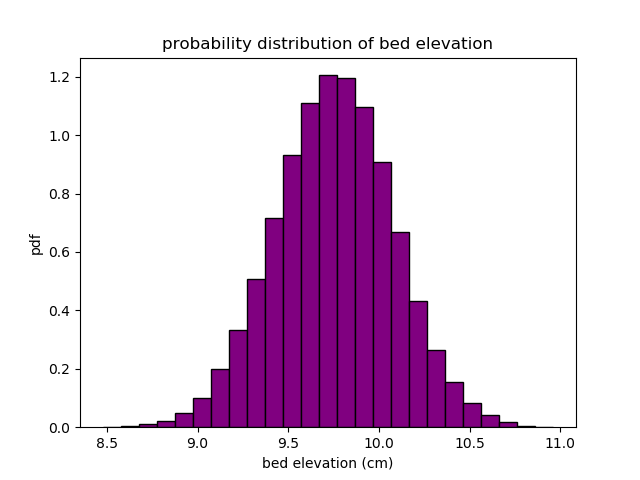
\includegraphics[width=0.45\textwidth]{elevationpdf.png} }}%
%    \caption{Particle activity and bed elevation probability distributions }%
%    \label{fig:example}%
%\end{figure}



\bibliography{biblio}


\end{document}
